\documentclass[a4paper, 12pt]{article}
\usepackage{graphicx}
\usepackage{ctex}
\usepackage{listings}  
\usepackage{xcolor}    

\lstset{
  basicstyle=\ttfamily\small,        
  keywordstyle=\color{blue},         
  commentstyle=\color{gray},         
  stringstyle=\color{red},           
  showstringspaces=false,            
  frame=single,                      
  numbers=left,                      
  numberstyle=\tiny\color{gray},     
  breaklines=true,                   
  linewidth=0.9\linewidth            
}

\begin{document}

\title{系统开发工具实验报告一}
\author{王子怡}
\date{\today}
\maketitle

\tableofcontents
\newpage 

% 第一部分:Git 指令
\part{Git 指令部分}

\section{git init}
\subsection{mkdir repository}
\label{sec1} 
创建目录
\subsection{git init}
使用 git init 初始化当前仓库\\ \\
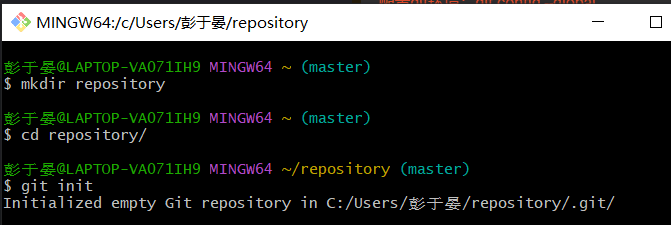
\includegraphics[width=1\linewidth]{1.png}

\section{git status}
显示当前的仓库状态\\ \\
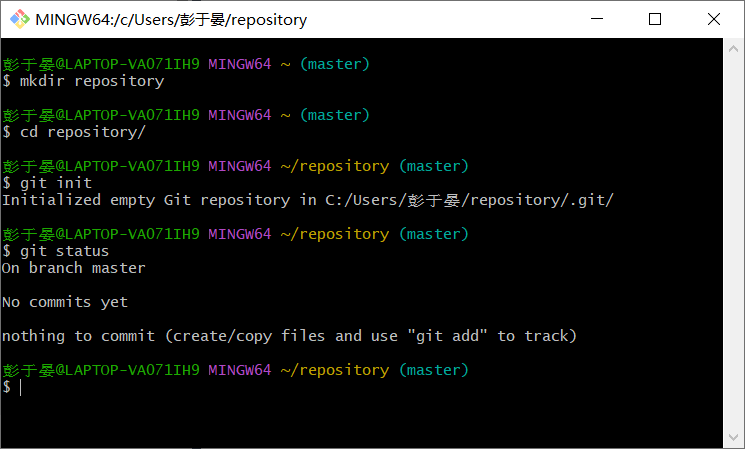
\includegraphics[width=1\linewidth]{2.png}  

\section{git add test.c}
添加文件到暂存区\\ \\
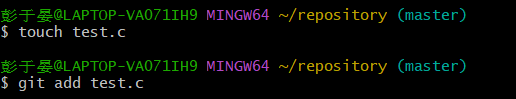
\includegraphics[width=1\linewidth]{3.png} 
  
\section{git commit -m "add new file \"test.c\""}
创建一个新的提交\\ \\
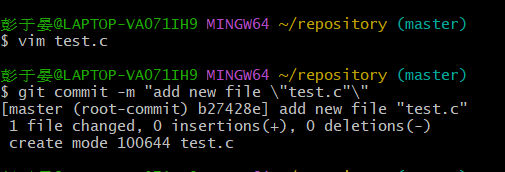
\includegraphics[width=1\linewidth]{4.png}
  
\section{git log}
显示日志\\ \\
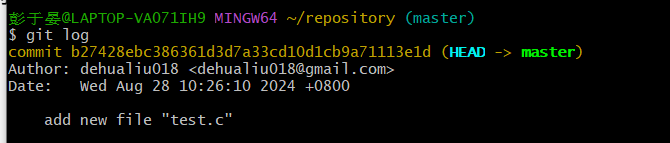
\includegraphics[width=1\linewidth]{5.png}
  
\section{git commit --amend}
改写上一次的提交信息\\ \\
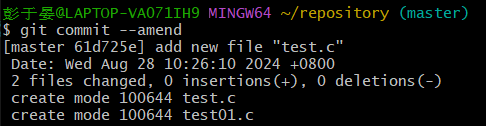
\includegraphics[width=1\linewidth]{6.png}
  
\section{git reset --hard -}
回滚代码仓库\\ \\
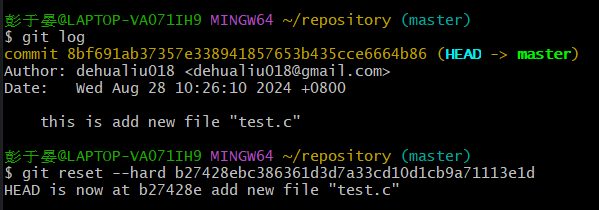
\includegraphics[width=1\linewidth]{7.png}
  
\section{git rm min.c}
删除提交的文件 \\ \\
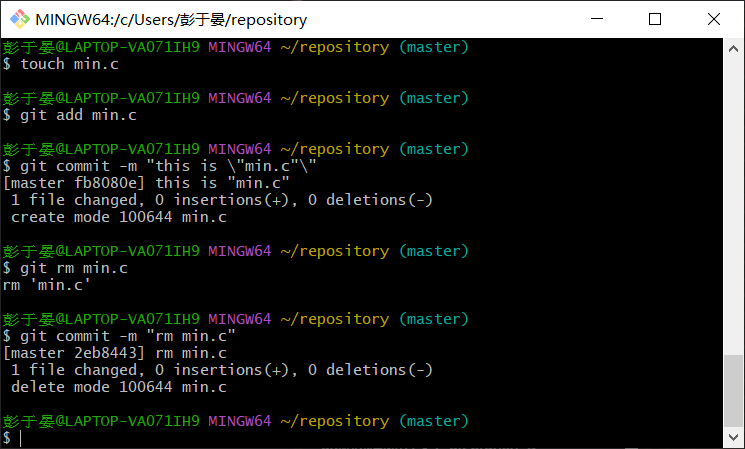
\includegraphics[width=1\linewidth]{8.png}
  
\section{git reflog}
查看提交历史\\ \\
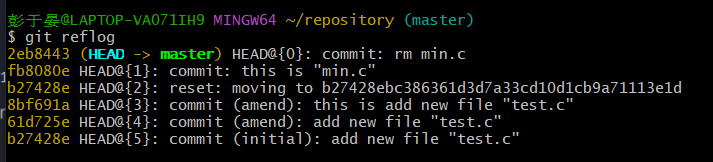
\includegraphics[width=1\linewidth]{9.png}

\section{git checkout -b dev}
使用 git checkout -b 参数来创建一个分支,创建完成分支后会自动切换过去\\ \\
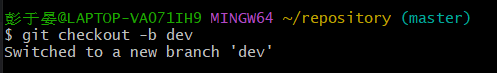
\includegraphics[width=1\linewidth]{10.png}

\section{git branch}
查看当前属于哪个分支\\ \\
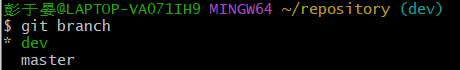
\includegraphics[width=1\linewidth]{11.png}

\section{git checkout master}
切换分支\\ \\
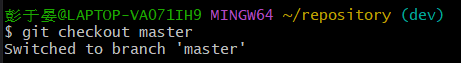
\includegraphics[width=1\linewidth]{12.png}

% 第二部分:LaTeX 用法
\part{LaTeX 用法部分}

\section{文档类声明}
\begin{lstlisting}[language=TeX]
\documentclass{article}  
%声明文档类型,例如 article, report, book 等
\end{lstlisting}

\section{标题与作者信息}
\begin{lstlisting}[language=TeX]
\title{Document Title}
\author{Author Name}
\date{\today}
\maketitle
%定义文档的标题、作者和日期。\today 自动插入当前日期,\maketitle 生成标题页,通常放在文档的开头部分。
\end{lstlisting}

\section{文本格式化}
\begin{lstlisting}[language=TeX]
\textbf{Bold Text} 
\textit{Italic Text} 
\underline{Underlined Text}
%用于格式化文本的命令。\textbf 使文字变为粗体,\textit 使文字变为斜体,\underline 为文字加下划线。可以在段落中任意位置使用。
\end{lstlisting}

\section{段落与换行}
\begin{lstlisting}[language=TeX]
% 空行表示段落换行
This is a new paragraph.
% 换行符
First line of text.\\
Second line of text.
%段落换行是通过插入一个空行实现的。\\ 用于在段落内换行,但不开始新段落。
\end{lstlisting}

\section{插入公式}
\begin{lstlisting}[language=TeX]
$E = mc^2$ 
\[ a^2 + b^2 = c^2 \]
%$...$ 表示行内公式,\[...\] 表示独立公式
\end{lstlisting}

\section{插入图像}
\begin{lstlisting}[language=TeX]
\usepackage{graphicx} 
\begin{figure}
\centering
\includegraphics[width=0.5\textwidth]{image.png}
\caption{Figure Caption}
\label{fig:sample}
\end{figure}
%\usepackage{graphicx} 导入 graphicx 包,使用 \includegraphics 命令。figure 环境用于包含图片,centering 用于居中显示,caption 设置图片标题,label 用于引用图片。
\end{lstlisting}

\section{创建表格}
\begin{lstlisting}[language=TeX]
\begin{tabular}{|c|c|c|}
\hline
A & B & C \\
\hline
1 & 2 & 3 \\
\hline
\end{tabular}
%tabular 环境用于定义表格的内容,|c|c|c| 表示三列居中对齐,并在每列之间和表格边缘绘制竖线,\hline 绘制水平线,& 分隔列内容,\\ 表示换行。
\end{lstlisting}

\section{引用与参考文献}
\begin{lstlisting}[language=TeX]
\usepackage{cite}  
文中引用 \cite{reference_key}。
\bibliographystyle{plain}
\bibliography{references}
%cite 命令引用指定文献(reference_key),\bibliographystyle 指定参考文献样式,\bibliography 引入文献数据库(references.bib 文件)。
\end{lstlisting}

\section{章节}
\begin{lstlisting}[language=TeX]
\section{Section Title}
\subsection{Subsection Title}
\subsubsection{Subsubsection Title}
%定义文档的层次结构。\section 创建一级标题,\subsection 创建二级标题,\subsubsection 创建三级标题。LaTeX 自动为这些标题编号,并包含在目录中。
\end{lstlisting}

\section{创建列表}
\begin{lstlisting}[language=TeX]
\begin{itemize}  
  \item First Item
  \item Second Item
\end{itemize}

\begin{enumerate}  
  \item First Item
  \item Second Item
\end{enumerate}
%创建无序和有序列表,itemize 环境用于无序列表,enumerate 环境用于有序列表,每个条目用 \item 开头。
\end{lstlisting}

\section{定义颜色}
\begin{lstlisting}[language=TeX]
\usepackage{xcolor}  
\textcolor{red}{Red Text}
%引入 xcolor 包支持文本着色,\textcolor 命令指定文本颜色,例如将文本设为红色。
\end{lstlisting}

\section{定义宏}
\begin{lstlisting}[language=TeX]
\newcommand{\R}{\mathbb{R}}
%自定义命令,使用 \newcommand 创建新的快捷命令 \R,它将在文档中表示为数学符号“实数集 R”。这样可以简化重复的复杂命令。
\end{lstlisting}

\end{document}
